\documentclass[a4paper, 12pt]{article}
\usepackage[utf8]{inputenc}
\usepackage[brazil]{babel}  
\usepackage[protrusion=true, expansion=true]{microtype}
\usepackage[hang, small, labelfont=bf, up, textfont=it, up]{caption}
\usepackage{graphicx}
\usepackage{fancyhdr}
\usepackage{hyperref}
\usepackage[a4paper, total={7in, 10in}]{geometry}
\usepackage[ddmmyyyy]{datetime}
\usepackage{lipsum}

\pagestyle{fancy}

\lhead{}
\chead{}
\rhead{}

\lfoot{Relatório de Análise de Dados do Integra UFMS 2019}
\cfoot{}
\rfoot{\footnotesize Folha \thepage\ }

\renewcommand{\headrulewidth}{0.0pt}
\renewcommand{\footrulewidth}{0.3pt}

%opening
\title{Relatório de Análise de Dados do Integra UFMS 2019}
\author{Daniel de Leon Bailo da Silva}

\begin{document}

\maketitle

\section{Introdução}\label{sec:introducao}
% Criado em 2017, o Integra UFMS é o maior evento de Ciência, Tecnologia, Inovação e Empreendedorismo do estado de Mato Grosso do Sul. O objetivo é reunir em um só local o resultado das atividades ligadas aos programas institucionais: Iniciação Científica, Iniciação à Docência, Educação Tutorial, Extensão Universitária, Mais Cultura, Esportes, Ensino de Graduação, Ligas Acadêmicas, Residência Pedagógica, Pós-Graduação Stricto Sensu, Empresas juniores e da Feira de Tecnologias, Engenharias e Ciências de Mato Grosso do Sul (Fetec-MS). Em 2018, mais de mil pôsteres foram apresentados e mais de 200 atividades foram realizadas, entre oficinas, workshops, palestras e minicursos.
Neste trabalho, tenho como objetivo, apresentar algumas estatísticas que foram obtidas a partir da análise e coleta de dados do Integra UFMS 2019.
\subsection{Materiais e Métodos}
Sabendo do evento, decidi realizar uma análise dos dados que foram obtivos atraves do EDITAL PROECE/PROGRAD/PROPP/AGINOVA Nº 59, DE 04 DE JUNHO DE 2019 SELEÇÃO DE TRABALHOS PARA APRESENTAÇÃO NO INTEGRA UFMS 2019 RESULTADO FINAL E DATA DE PROGRAMAÇÃO.

Desenvolvi um programa para ler este documento em pdf, onde o mesmo, só iria pegar do documento as coisas que me interessavam, que no caso era as tabelas onde continham os seguintes dados: Estudante, Unidade, Título do Trabalho, Programa e Data da apresentação.

Feito isso, organizei os dados em um {\it DataFrame}, e daí, eu consigo extrair qualquer coisa que seja relevante saber, por exemplo: o número total de trabalhos enviados, qual foi o campus que mais submeteu trabalhos, quantos trabalhos cada aluno submeteu, etc.

\newpage
\section{Análise Descritiva dos Dados}
Como podemos ver, o Campus que mais submeteu trabalhos foi o Campus de Três Lagoas, com um total de 162 projetos, dividos em ensino, pesquisa e extensão.
\vspace{-30pt}
\begin{figure}[h]
	\centering
	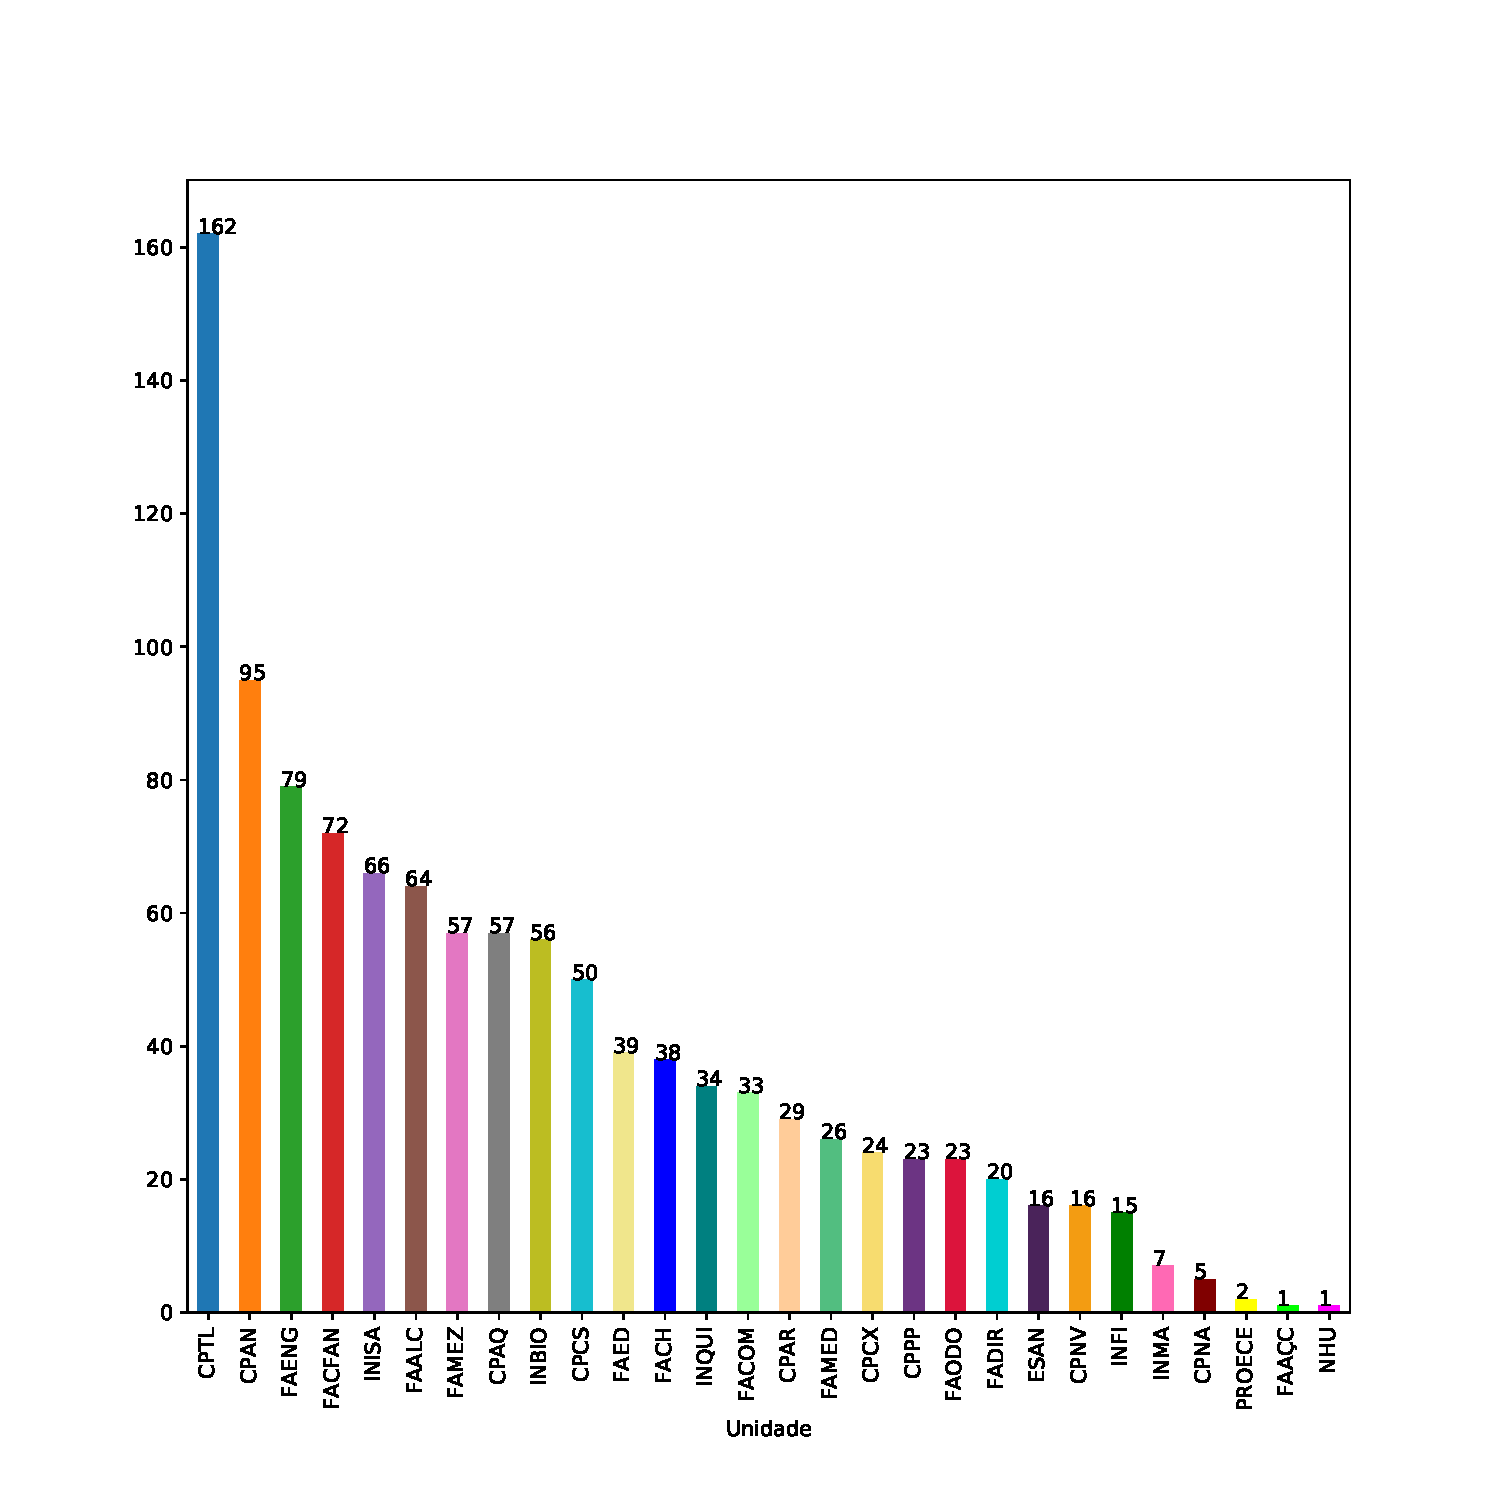
\includegraphics[width=1\textwidth]{../img/unidade_bar.pdf}
	\caption{Gráfico do número de trabalho submetidos por Campus}
	\label{}
\end{figure}
\newpage

Com isso, somente o Campus de Três Lagoas, preenche um total de $14.6\%$...
\begin{figure}[h]
	\centering
	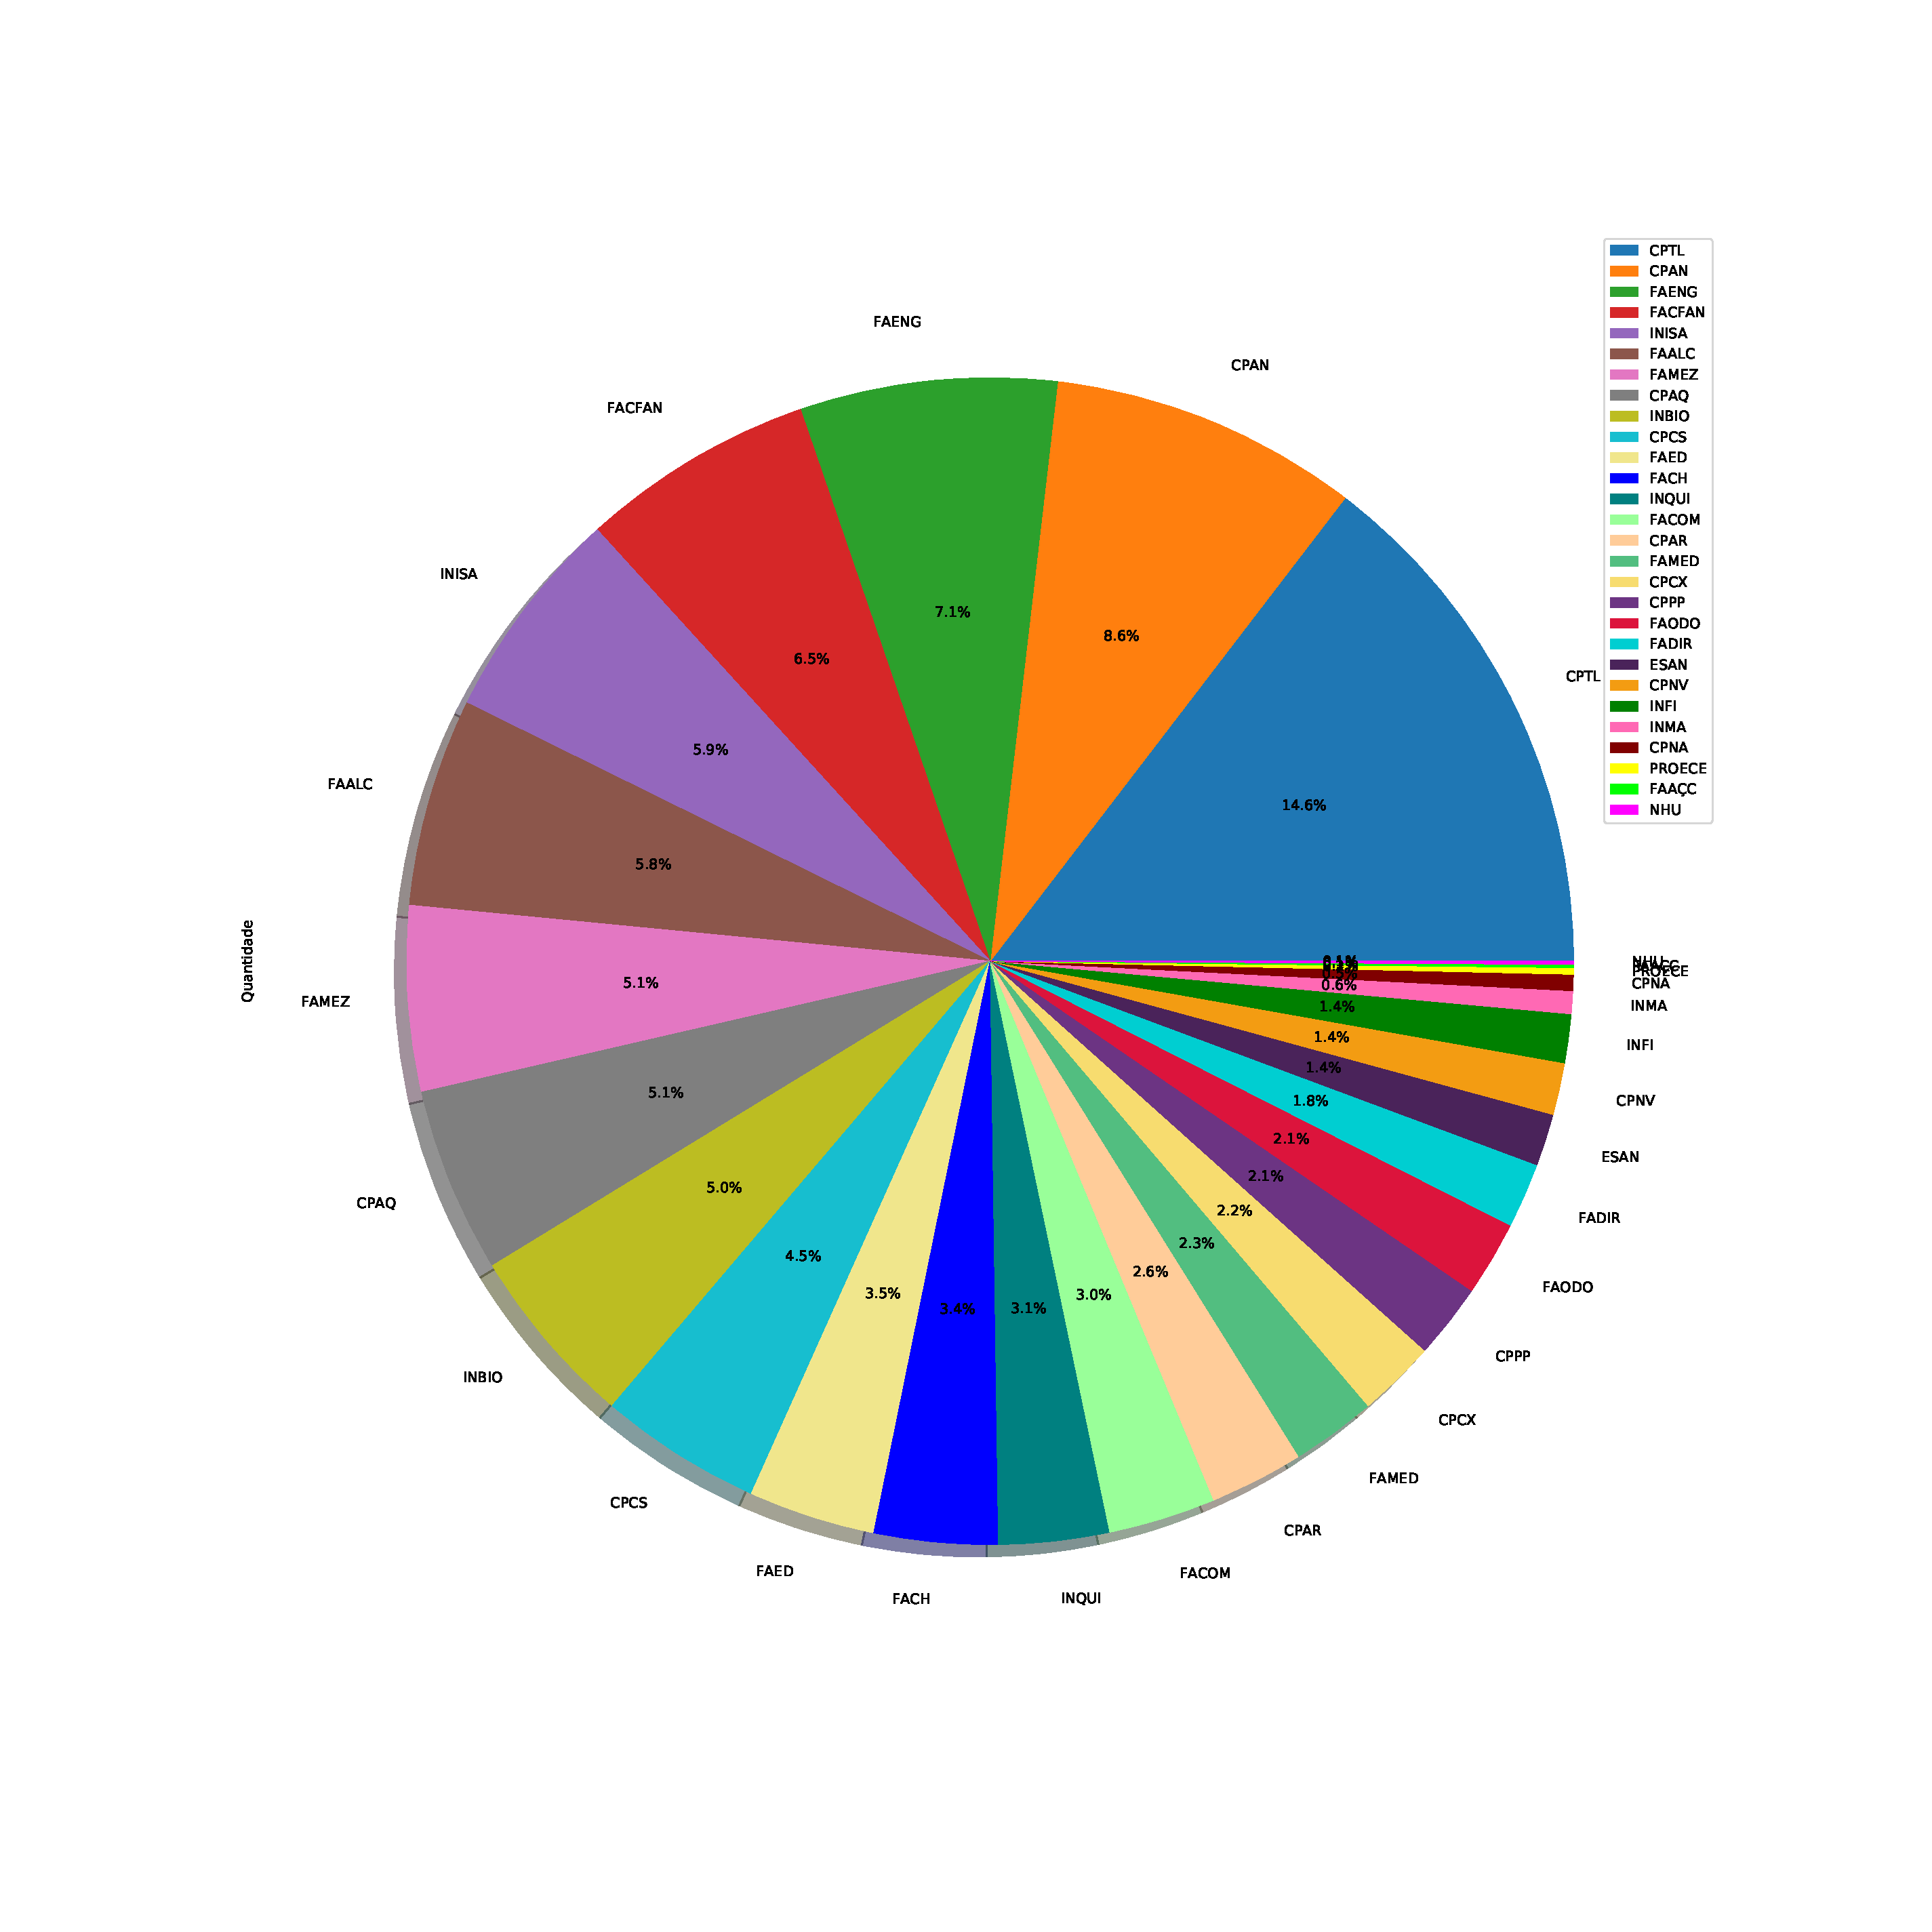
\includegraphics[width=0.9\textwidth]{../img/unidade_pie.pdf}
	\caption{Gráfico do número de trabalho submetidos por Campus}
	\label{}
\end{figure}
\newpage

Como podemos ver, o Campus que mais submeteu trabalhos foi o Campus de Três Lagoas, com um total de 162 projetos, dividos em ensino, pesquisa e extensão.
\vspace{-30pt}
\begin{figure}[h]
	\centering
	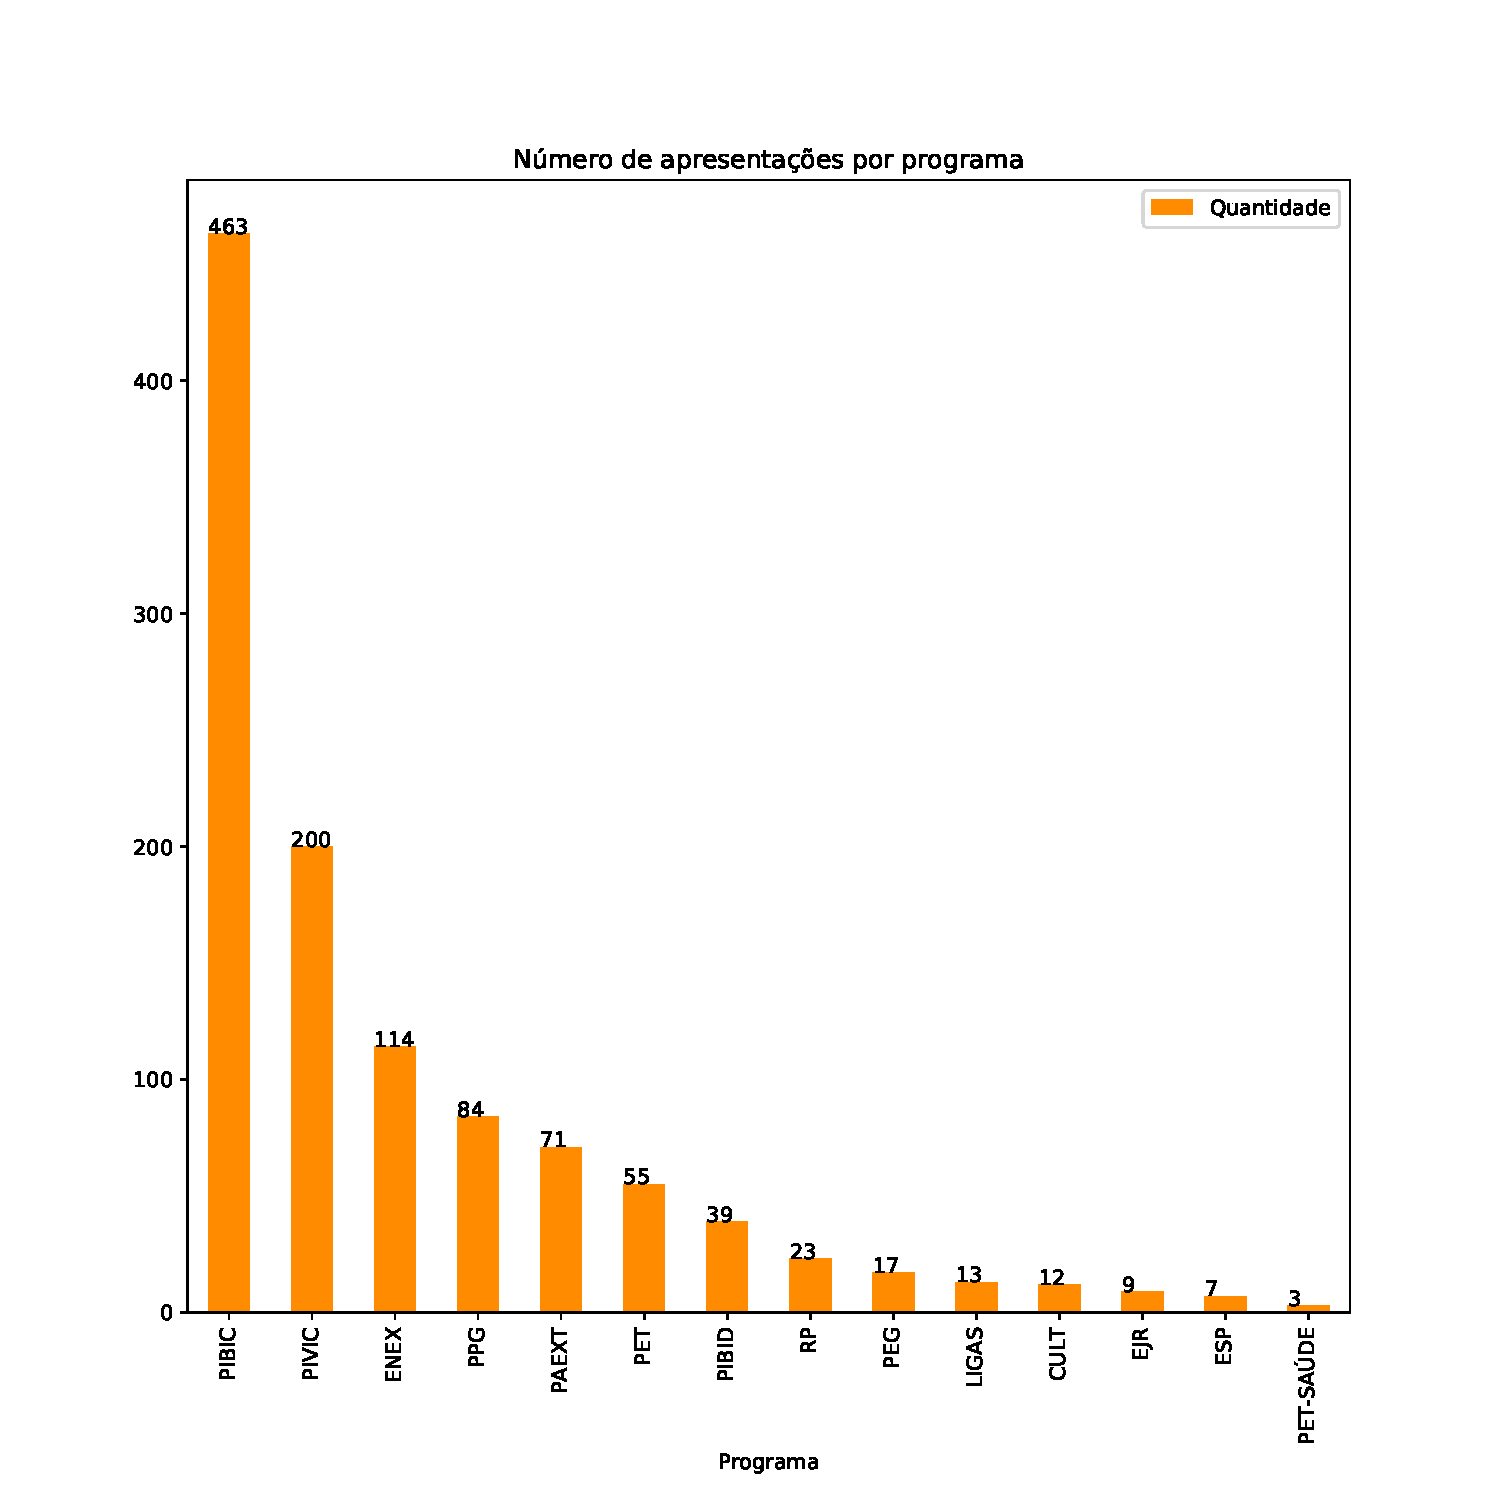
\includegraphics[width=1\textwidth]{../img/programa_bar.pdf}
	\caption{Gráfico do número de trabalho submetidos por programa}
	\label{}
\end{figure}
\newpage

Com isso, somente o Campus de Três Lagoas, preenche um total de $14.6\%$...
\begin{figure}[h]
	\centering
	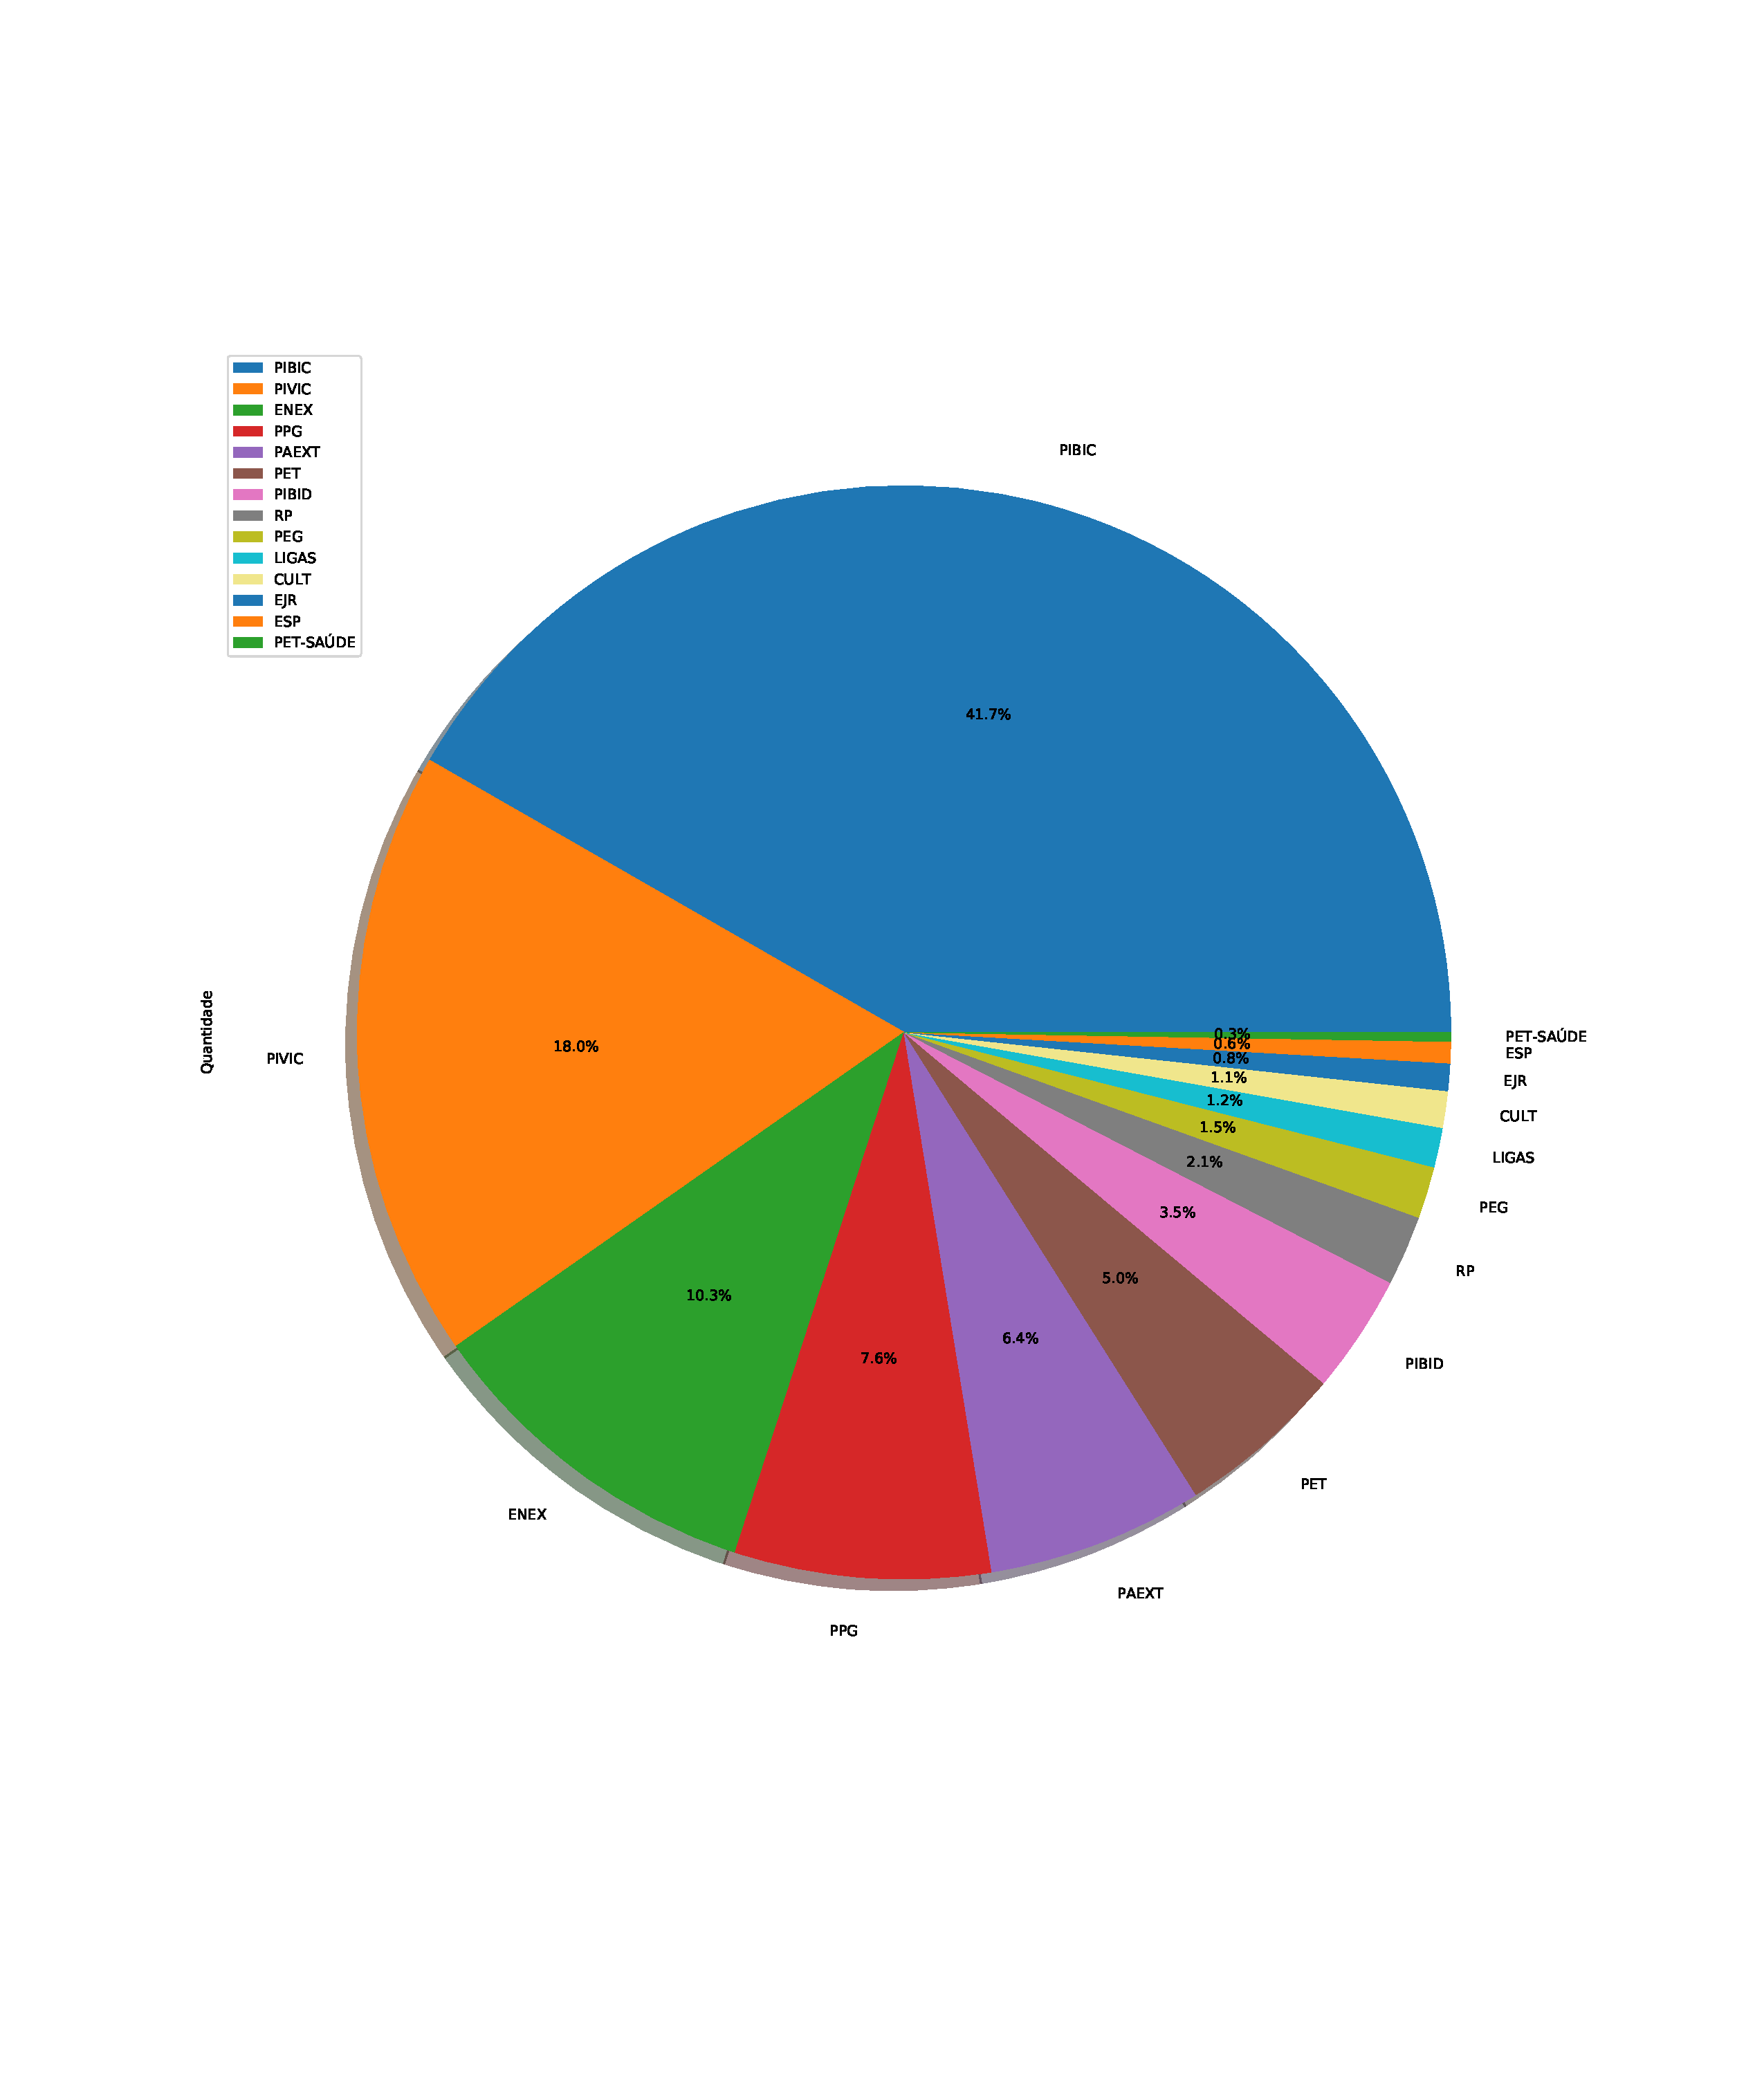
\includegraphics[width=0.9\textwidth]{../img/programa_pie.pdf}
	\caption{Gráfico do número de trabalho submetidos por Campus}
	\label{}
\end{figure}
\newpage

\section{Conclusão}
\lipsum[3]

\end{document}
